\documentclass[aspectratio=169,10pt]{beamer}
\usepackage[utf8]{inputenc}
\usepackage[T1]{fontenc}
\usepackage[polish]{babel}
\usepackage{lmodern}
\usepackage{booktabs}
\usepackage{tabularx}
\usepackage{array}

\usetheme{default}
\usecolortheme{default}
\setbeamertemplate{navigation symbols}{}
\setbeamertemplate{footline}[frame number]
\definecolor{smblue}{HTML}{2F6DB5}
\setbeamercolor{frametitle}{fg=smblue}
\setbeamercolor{title}{fg=smblue}
\setbeamercolor{structure}{fg=smblue}

\graphicspath{{../docs/diagrams/png/}}
\newcolumntype{L}{>{\raggedright\arraybackslash}X}

\title{SkillMatrix}
\subtitle{Historie użytkownika, przypadki użycia i diagramy klas}
\author{Jan Kaszycki \and Aleksandr Kuraskin}
\date{Inżynieria Oprogramowania 1 --- 2026}

\begin{document}

\begin{frame}
  \titlepage
\end{frame}

% ------------------------------------------------------------------
\begin{frame}{Problem i pomysł}
  \textbf{Problem:} kandydat nie wie, jak jego umiejętności mają się do wymagań rynku.
  CV opisuje je ogólnikowo, oferty --- każda po swojemu, a porównanie robi się ręcznie.

  \bigskip
  \textbf{SkillMatrix:}
  \begin{itemize}
    \item umiejętności jako \alert{graf atomowych umiejętności}, każda z poziomem 0--1,
    \item poziom szacuje \alert{AI} na podstawie CV, ocen i kodu z GitHuba,
    \item oferty \alert{pobieramy automatycznie z portali}, a AI zamienia je na ten sam graf,
    \item system wskazuje dopasowane oferty, braki i \alert{czego się nauczyć},
    \item ocena i generowanie CV.
  \end{itemize}

  \bigskip
  Poziomy pokazujemy opisowo (Początkujący \dots\ Ekspert). Jeśli kandydat bardzo chce,
  może włączyć liczby i poprawić ocenę AI ręcznie --- ale tego nie zalecamy.
\end{frame}

% ------------------------------------------------------------------
\begin{frame}{Kto i co działa w systemie}
  \small
  \begin{tabularx}{\textwidth}{@{}>{\bfseries\raggedright\arraybackslash}p{3.1cm} p{2.3cm} L@{}}
    \toprule
    Aktor & Rodzaj & Co robi \\
    \midrule
    Kandydat & człowiek & Wgrywa CV, oceny, link do GitHuba; ogląda swój graf, oferty, rekomendacje, CV. Jedyny człowiek w systemie. \\
    Serwer SkillMatrix & nasz program & Trzyma konta, profile, oferty i graf; liczy dopasowanie i rekomendacje. \\
    Agent ofert & nasz program & Robot: według harmonogramu pobiera ogłoszenia z portali z pracą i oddaje je serwerowi. Nie używa AI. \\
    Agent AI & nasz program & „Mózg”: ocenia umiejętności kandydata, zamienia treść ofert na umiejętności z grafu, ocenia CV. \alert{Pełni rolę administratora grafu} --- dodaje węzły, scala duplikaty. \\
    Model językowy (LLM) & zewnętrzny & Np.\ Claude API: dostaje tekst i instrukcję, zwraca JSON. Używa go tylko Agent AI. \\
    GitHub API, portale & zewnętrzne & Źródła danych o kodzie kandydata i ofert pracy. \\
    \bottomrule
  \end{tabularx}

  \medskip
  Nie ma rekruterów ani administratora-człowieka.
\end{frame}

% ------------------------------------------------------------------
\begin{frame}{Historie użytkownika --- Kandydat}
  \footnotesize
  \begin{tabularx}{\textwidth}{@{}l L c@{}}
    \toprule
    ID & Jako \emph{kandydat} chcę \dots, aby \dots & Prio \\
    \midrule
    US-02/03 & wgrać CV i oceny, aby system poznał moje doświadczenie bez przepisywania & M \\
    US-04 & podać link do profilu lub repozytorium GitHub, aby ocena opierała się na faktycznym kodzie & M \\
    US-05 & żeby AI oszacowało moje umiejętności 0--1, aby dostać mierzalny obraz tego, co umiem & M \\
    US-06 & widzieć graf z poziomem opisowym i uzasadnieniem, aby rozumieć ocenę bez fiksowania się na liczbach & M \\
    US-07 & móc (niezalecane) włączyć liczby i poprawić ocenę AI, aby skorygować ocenę, z którą się nie zgadzam & C \\
    US-08 & widzieć oferty posortowane wg dopasowania, aby aplikować tam, gdzie mam szanse & M \\
    US-09 & widzieć braki dla wybranej oferty, aby wiedzieć, co dzieli mnie od tej pracy & M \\
    US-11 & dostać umiejętności, które odblokują najwięcej ofert, aby uczyć się tego, co się opłaca & M \\
    US-13/14 & ocenić i wygenerować CV, aby lepiej pokazać, co umiem & S \\
    \bottomrule
  \end{tabularx}
\end{frame}

% ------------------------------------------------------------------
\begin{frame}{Historie użytkownika --- Agent AI i Agent ofert}
  \footnotesize
  \begin{tabularx}{\textwidth}{@{}l L c@{}}
    \toprule
    ID & Historia & Prio \\
    \midrule
    US-20 & Jako \emph{agent AI} chcę zamieniać treść ogłoszenia na wymagania z grafu (poziom, obowiązkowe?), aby oferty dało się porównać z profilami & M \\
    US-21 & Jako \emph{agent AI} chcę przed dodaniem umiejętności sprawdzić, czy nie istnieje pod inną nazwą, aby w grafie nie było duplikatów & M \\
    US-22 & Jako \emph{agent AI} chcę dodawać nowe umiejętności jako tymczasowe, aby jednorazowe pomyłki nie zaśmiecały grafu & S \\
    US-23 & Jako \emph{agent AI} chcę okresowo scalać duplikaty, aby naprawić te, które przeszły przy dodawaniu & S \\
    US-24 & Jako \emph{agent AI} chcę wyznaczać relacje (C++ $\ge 0.8 \Rightarrow$ C $\ge 0.6$), aby wnioskować o umiejętnościach pokrewnych & S \\
    \midrule
    US-30 & Jako \emph{agent ofert} chcę cyklicznie pobierać ogłoszenia z portali, aby baza ofert była aktualna bez udziału człowieka & M \\
    US-31 & Jako \emph{agent ofert} chcę rozpoznawać tę samą ofertę z różnych portali, aby kandydat nie widział jej kilka razy & S \\
    US-32 & Jako \emph{agent ofert} chcę oznaczać zniknięte oferty jako nieaktualne, aby kandydat nie widział wygasłych & S \\
    \bottomrule
  \end{tabularx}
\end{frame}

% ------------------------------------------------------------------
\begin{frame}{Przypadki użycia --- Profil umiejętności}
  \centering
  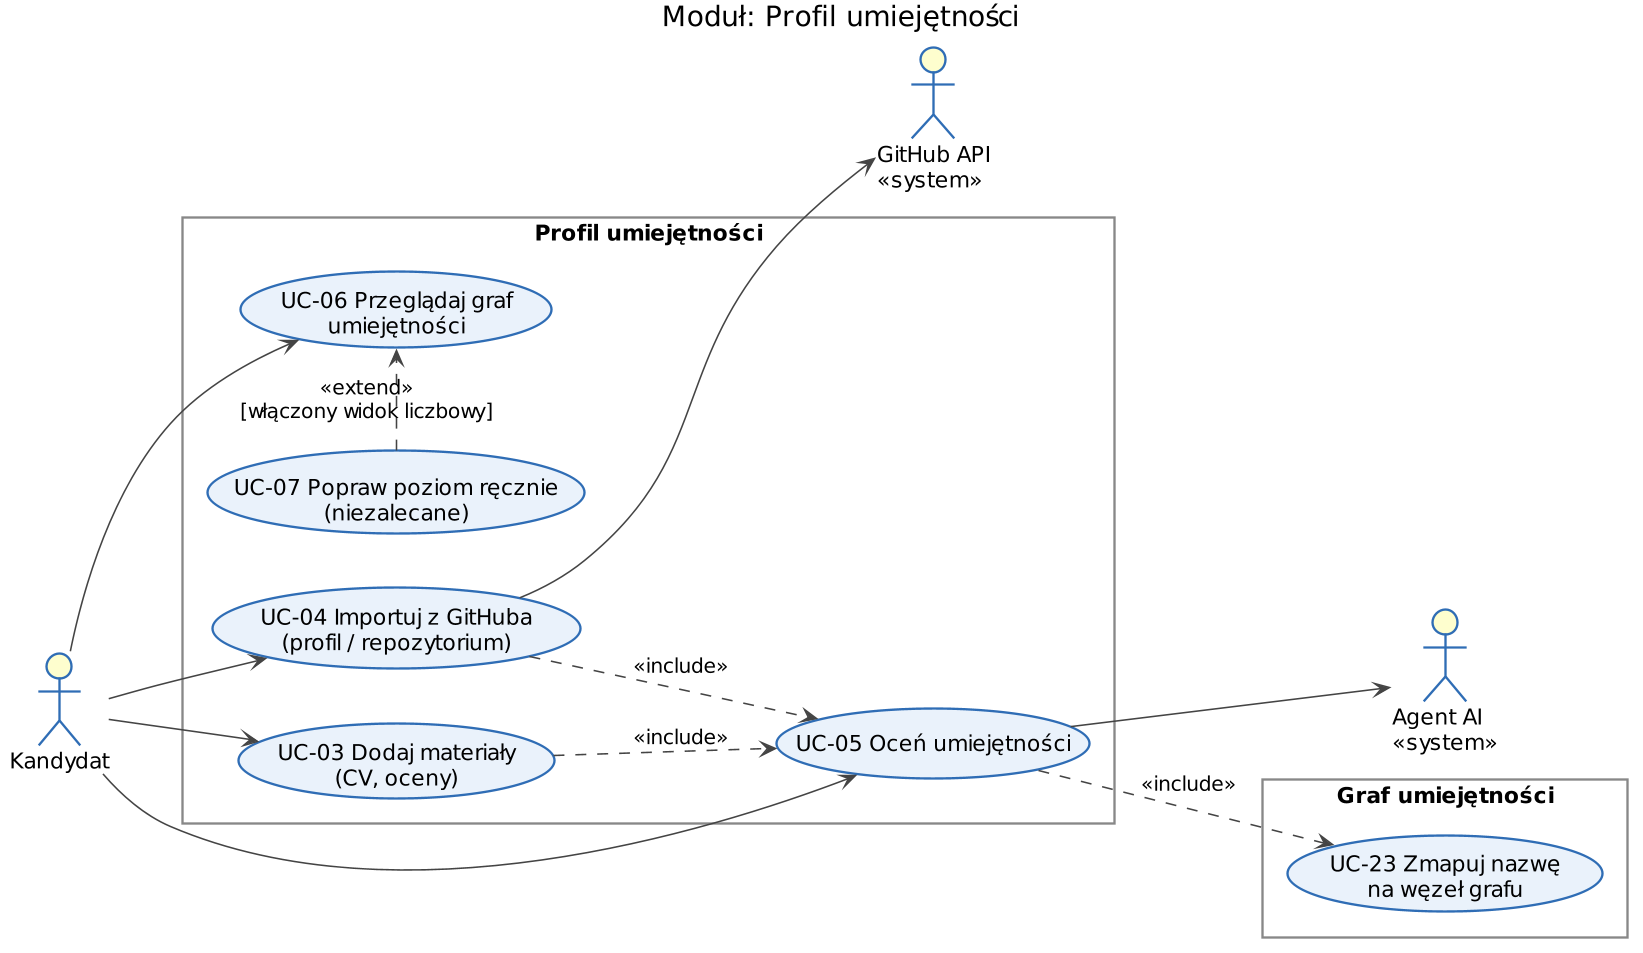
\includegraphics[width=\textwidth,height=0.82\textheight,keepaspectratio]{uc-profile}
\end{frame}

\begin{frame}{UC-05 Oceń umiejętności}
  \scriptsize
  \begin{tabularx}{\textwidth}{@{}>{\bfseries}p{2.6cm} L@{}}
    \toprule
    Aktorzy & Kandydat (główny), Agent AI \\
    Wyzwalacz & Dodanie materiału (UC-03, UC-04) lub „oceń ponownie” \\
    Warunek wstępny & Kandydat zalogowany, ma co najmniej jeden materiał \\
    Warunek końcowy & Profil ma poziom, pewność i uzasadnienie dla każdej umiejętności; zdarzenie \texttt{ProfileUpdated} \\
    \midrule
    Scenariusz główny &
      1.~System zbiera materiały kandydata (CV, oceny, GitHub).
      2.~Wysyła je do Agenta AI.
      3.~Agent AI zwraca oszacowania (nazwa, poziom 0--1, pewność, uzasadnienie).
      4.~Każda nazwa jest mapowana na węzeł grafu (UC-23).
      5.~System propaguje poziomy po relacjach \texttt{IMPLIES}.
      6.~Zapisuje ocenę i aktualizuje profil.
      7.~Pokazuje graf z poziomami opisowymi. \\
    Alternatywy &
      6a.~Kandydat ręcznie poprawił poziom $\rightarrow$ nowa wartość AI zapisana obok, korekta nie jest nadpisywana.
      7a.~Włączony widok liczbowy $\rightarrow$ dodatkowo wartości 0--1. \\
    \midrule
    Błędy & Agent AI / LLM niedostępny, timeout 60\,s; niepoprawny format odpowiedzi \\
    Stan po błędzie & Profil bez zmian, materiały zapisane, komunikat „spróbuj później” \\
    \bottomrule
  \end{tabularx}
\end{frame}

% ------------------------------------------------------------------
\begin{frame}{Przypadki użycia --- Oferty pracy}
  \centering
  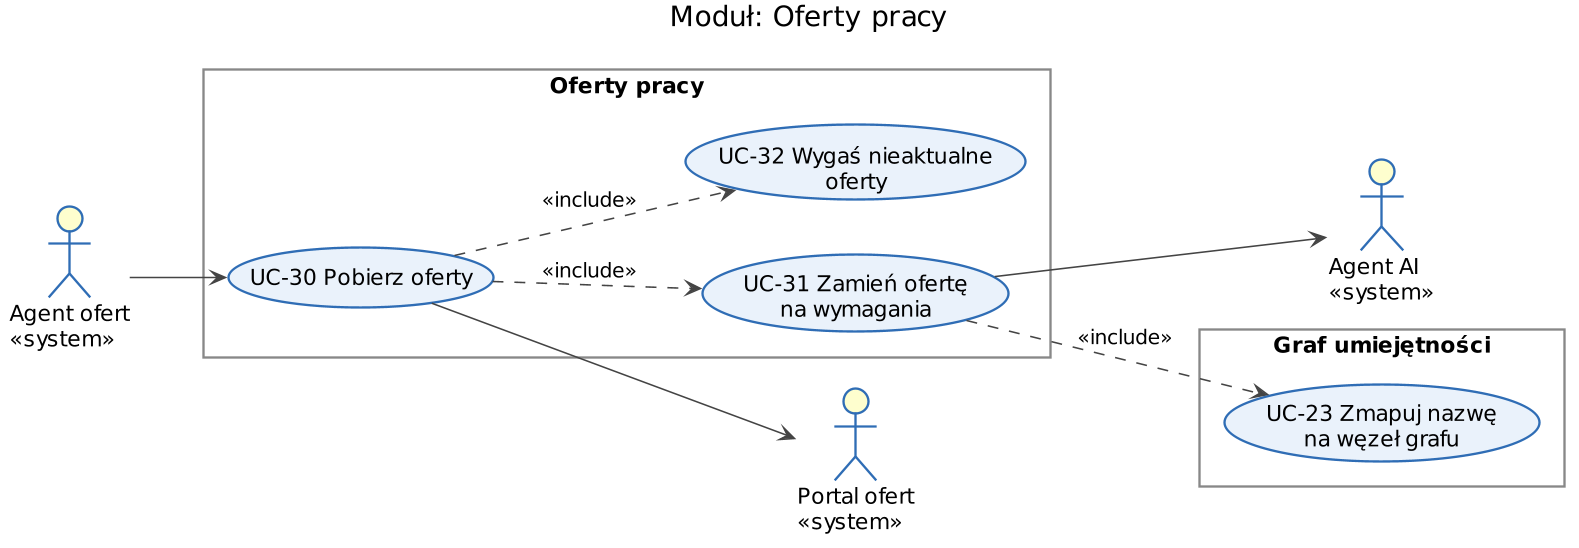
\includegraphics[width=\textwidth,height=0.82\textheight,keepaspectratio]{uc-offers}
\end{frame}

\begin{frame}{UC-30 Pobierz oferty}
  \scriptsize
  \begin{tabularx}{\textwidth}{@{}>{\bfseries}p{2.6cm} L@{}}
    \toprule
    Aktorzy & Agent ofert (główny), Portal ofert, Agent AI \\
    Wyzwalacz & Termin z harmonogramu źródła (plik konfiguracyjny) \\
    Warunek wstępny & Źródło ofert skonfigurowane i włączone \\
    Warunek końcowy & Oferty dodane / zaktualizowane / wygaszone; zapisany \texttt{IngestionRun}; zdarzenie \texttt{OffersUpdated} \\
    \midrule
    Scenariusz główny &
      1.~Agent ofert pobiera listę włączonych źródeł.
      2.~Pobiera ogłoszenia od ostatniego przebiegu (adapter API / scraper).
      3.~Odrzuca duplikaty (\texttt{externalId}, odcisk treści).
      4.~Agent AI zamienia każdą nową ofertę na wymagania z grafu (UC-31, UC-23).
      5.~Agent ofert przesyła paczkę do serwera (\texttt{upsertOffers}).
      6.~Serwer wygasza oferty, których już nie ma (UC-32).
      7.~Agent zapisuje raport przebiegu. \\
    Alternatywy &
      3a.~Zmieniona treść istniejącej oferty $\rightarrow$ ponowne wyodrębnienie wymagań.
      4a.~Brak rozpoznanych wymagań $\rightarrow$ oferta zapisana, ale pominięta w dopasowaniu. \\
    \midrule
    Błędy & Portal niedostępny lub zmienił strukturę; Agent AI niedostępny \\
    Stan po błędzie & Pozostałe źródła działają dalej; błąd w logu; oferty z tego źródła nie są wygaszane \\
    \bottomrule
  \end{tabularx}
\end{frame}

% ------------------------------------------------------------------
\begin{frame}{Przypadki użycia --- Graf umiejętności (zarządza Agent AI)}
  \centering
  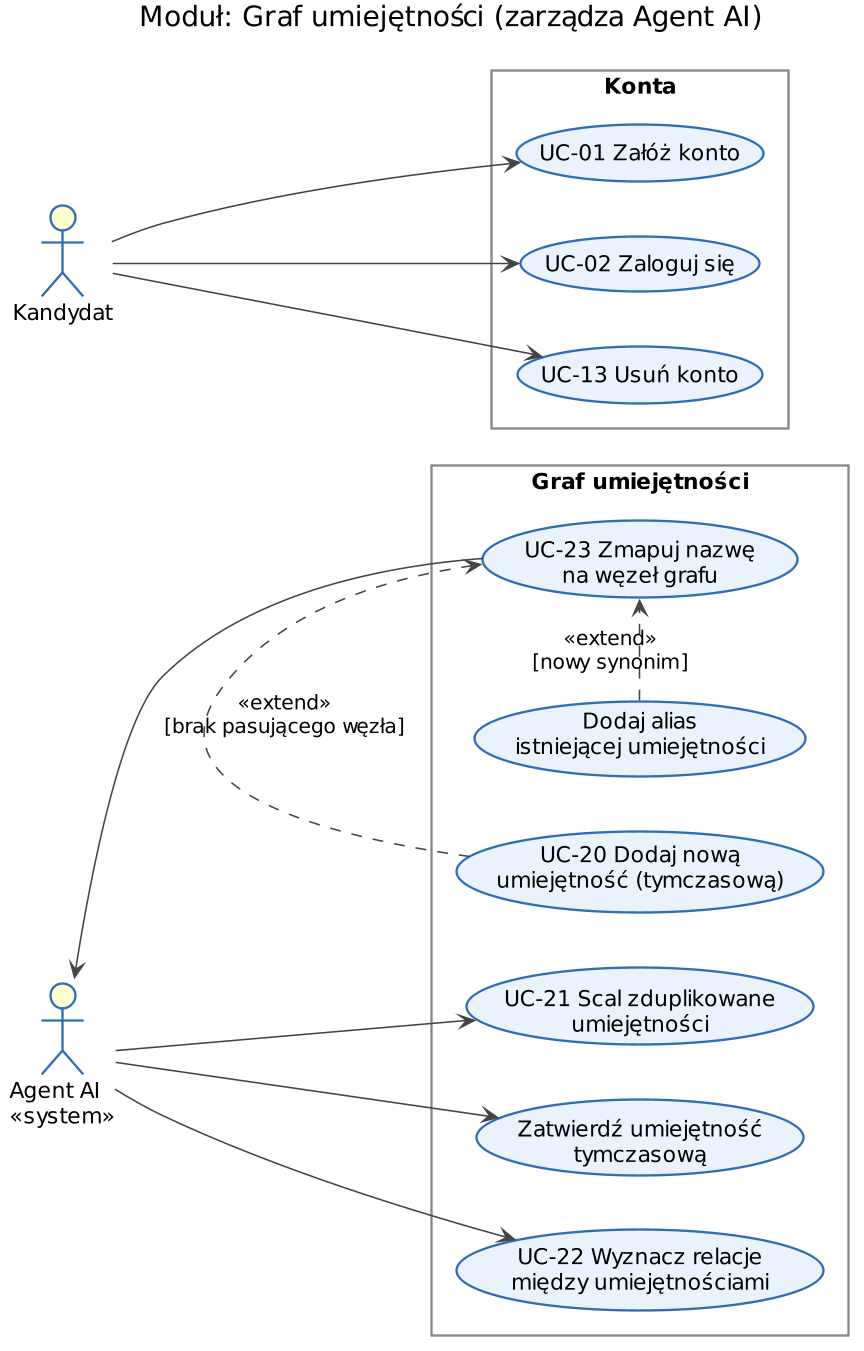
\includegraphics[width=\textwidth,height=0.82\textheight,keepaspectratio]{uc-graph}
\end{frame}

\begin{frame}{Problem: AI może tworzyć niejednoznaczne węzły}
  \small
  \begin{columns}[T]
    \begin{column}{0.42\textwidth}
      \textbf{Co może pójść źle}
      \begin{itemize}
        \item synonimy: \emph{JS} / \emph{JavaScript}
        \item pisownia, wersje: \emph{ReactJS} / \emph{React 18}
        \item język: \emph{bazy danych} / \emph{databases}
        \item szczegółowość: \emph{React} / \emph{React Hooks}
        \item ta sama oferta $\rightarrow$ różne nazwy
        \item „praca w zespole” jako węzeł
      \end{itemize}
      \medskip
      Skutek: kandydat z \emph{JavaScript} nie pasuje do oferty z \emph{JS}.
    \end{column}
    \begin{column}{0.56\textwidth}
      \textbf{Jak zapobiegamy}
      \begin{enumerate}
        \item AI \alert{najpierw wybiera z istniejących węzłów}, nowy to ostateczność (UC-23)
        \item normalizacja nazw + \alert{aliasy} zamiast nowych węzłów
        \item podobieństwo znaczeniowe (embeddingi): $\ge 0.92$ alias, $0.75$--$0.92$ decyduje LLM wybierając z listy, $< 0.75$ nowy węzeł
        \item graf startowy z gotowej klasyfikacji (np.\ ESCO)
        \item temperatura 0, stałe prompty, odpowiedź wg schematu JSON
        \item nowy węzeł \alert{tymczasowy} do czasu wystąpienia w $\ge 3$ ofertach
        \item nocne scalanie duplikatów + dziennik zmian z możliwością cofnięcia
      \end{enumerate}
    \end{column}
  \end{columns}
\end{frame}

\begin{frame}{UC-23 Zmapuj nazwę na węzeł grafu}
  \scriptsize
  \begin{tabularx}{\textwidth}{@{}>{\bfseries}p{2.6cm} L@{}}
    \toprule
    Aktorzy & Agent AI \\
    Wyzwalacz & Krok UC-05 lub UC-31 --- pojawia się nazwa umiejętności do zapisania \\
    Warunek wstępny & Graf zawiera węzły z aliasami i wektorami podobieństwa \\
    Warunek końcowy & Nazwa wskazuje dokładnie jeden węzeł; ewentualna zmiana grafu zapisana w dzienniku z uzasadnieniem \\
    \midrule
    Scenariusz główny &
      1.~Agent normalizuje nazwę (małe litery, bez wersji, kropek, myślników).
      2.~Szuka węzła o tej nazwie lub aliasie --- znaleziony: koniec.
      3.~Liczy embedding nazwy z kontekstem i pobiera 5 najbardziej podobnych węzłów.
      4.~Podobieństwo najlepszego $\ge 0.92$: dodaje nazwę jako alias i zwraca ten węzeł. \\
    Alternatywy &
      4a.~Podobieństwo $0.75$--$0.92$: LLM wybiera węzeł z listy kandydatów albo „nowa” $\rightarrow$ alias.
      4b.~$< 0.75$ lub „nowa”: tworzony węzeł \texttt{PROVISIONAL} (UC-20).
      4c.~LLM uznaje nazwę za nie-umiejętność $\rightarrow$ odrzucona. \\
    \midrule
    Błędy & LLM niedostępny w kroku 4a \\
    Stan po błędzie & Nazwa w kolejce do ponownego przetworzenia; graf bez zmian \\
    \bottomrule
  \end{tabularx}
\end{frame}

% ------------------------------------------------------------------
\begin{frame}{Przypadki użycia --- Dopasowanie, rekomendacje, CV}
  \centering
  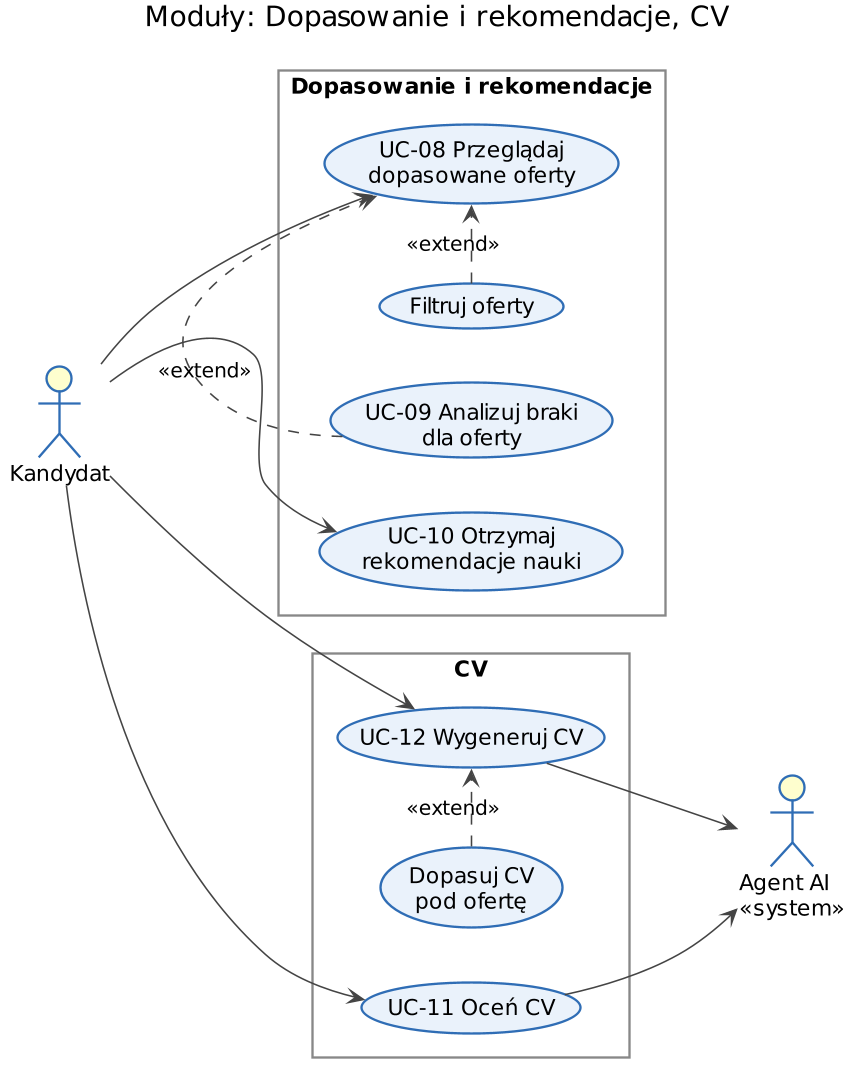
\includegraphics[width=\textwidth,height=0.82\textheight,keepaspectratio]{uc-matching}
\end{frame}

% ------------------------------------------------------------------
\begin{frame}{Diagram klas --- moduły i serwisy komunikacji}
  \centering
  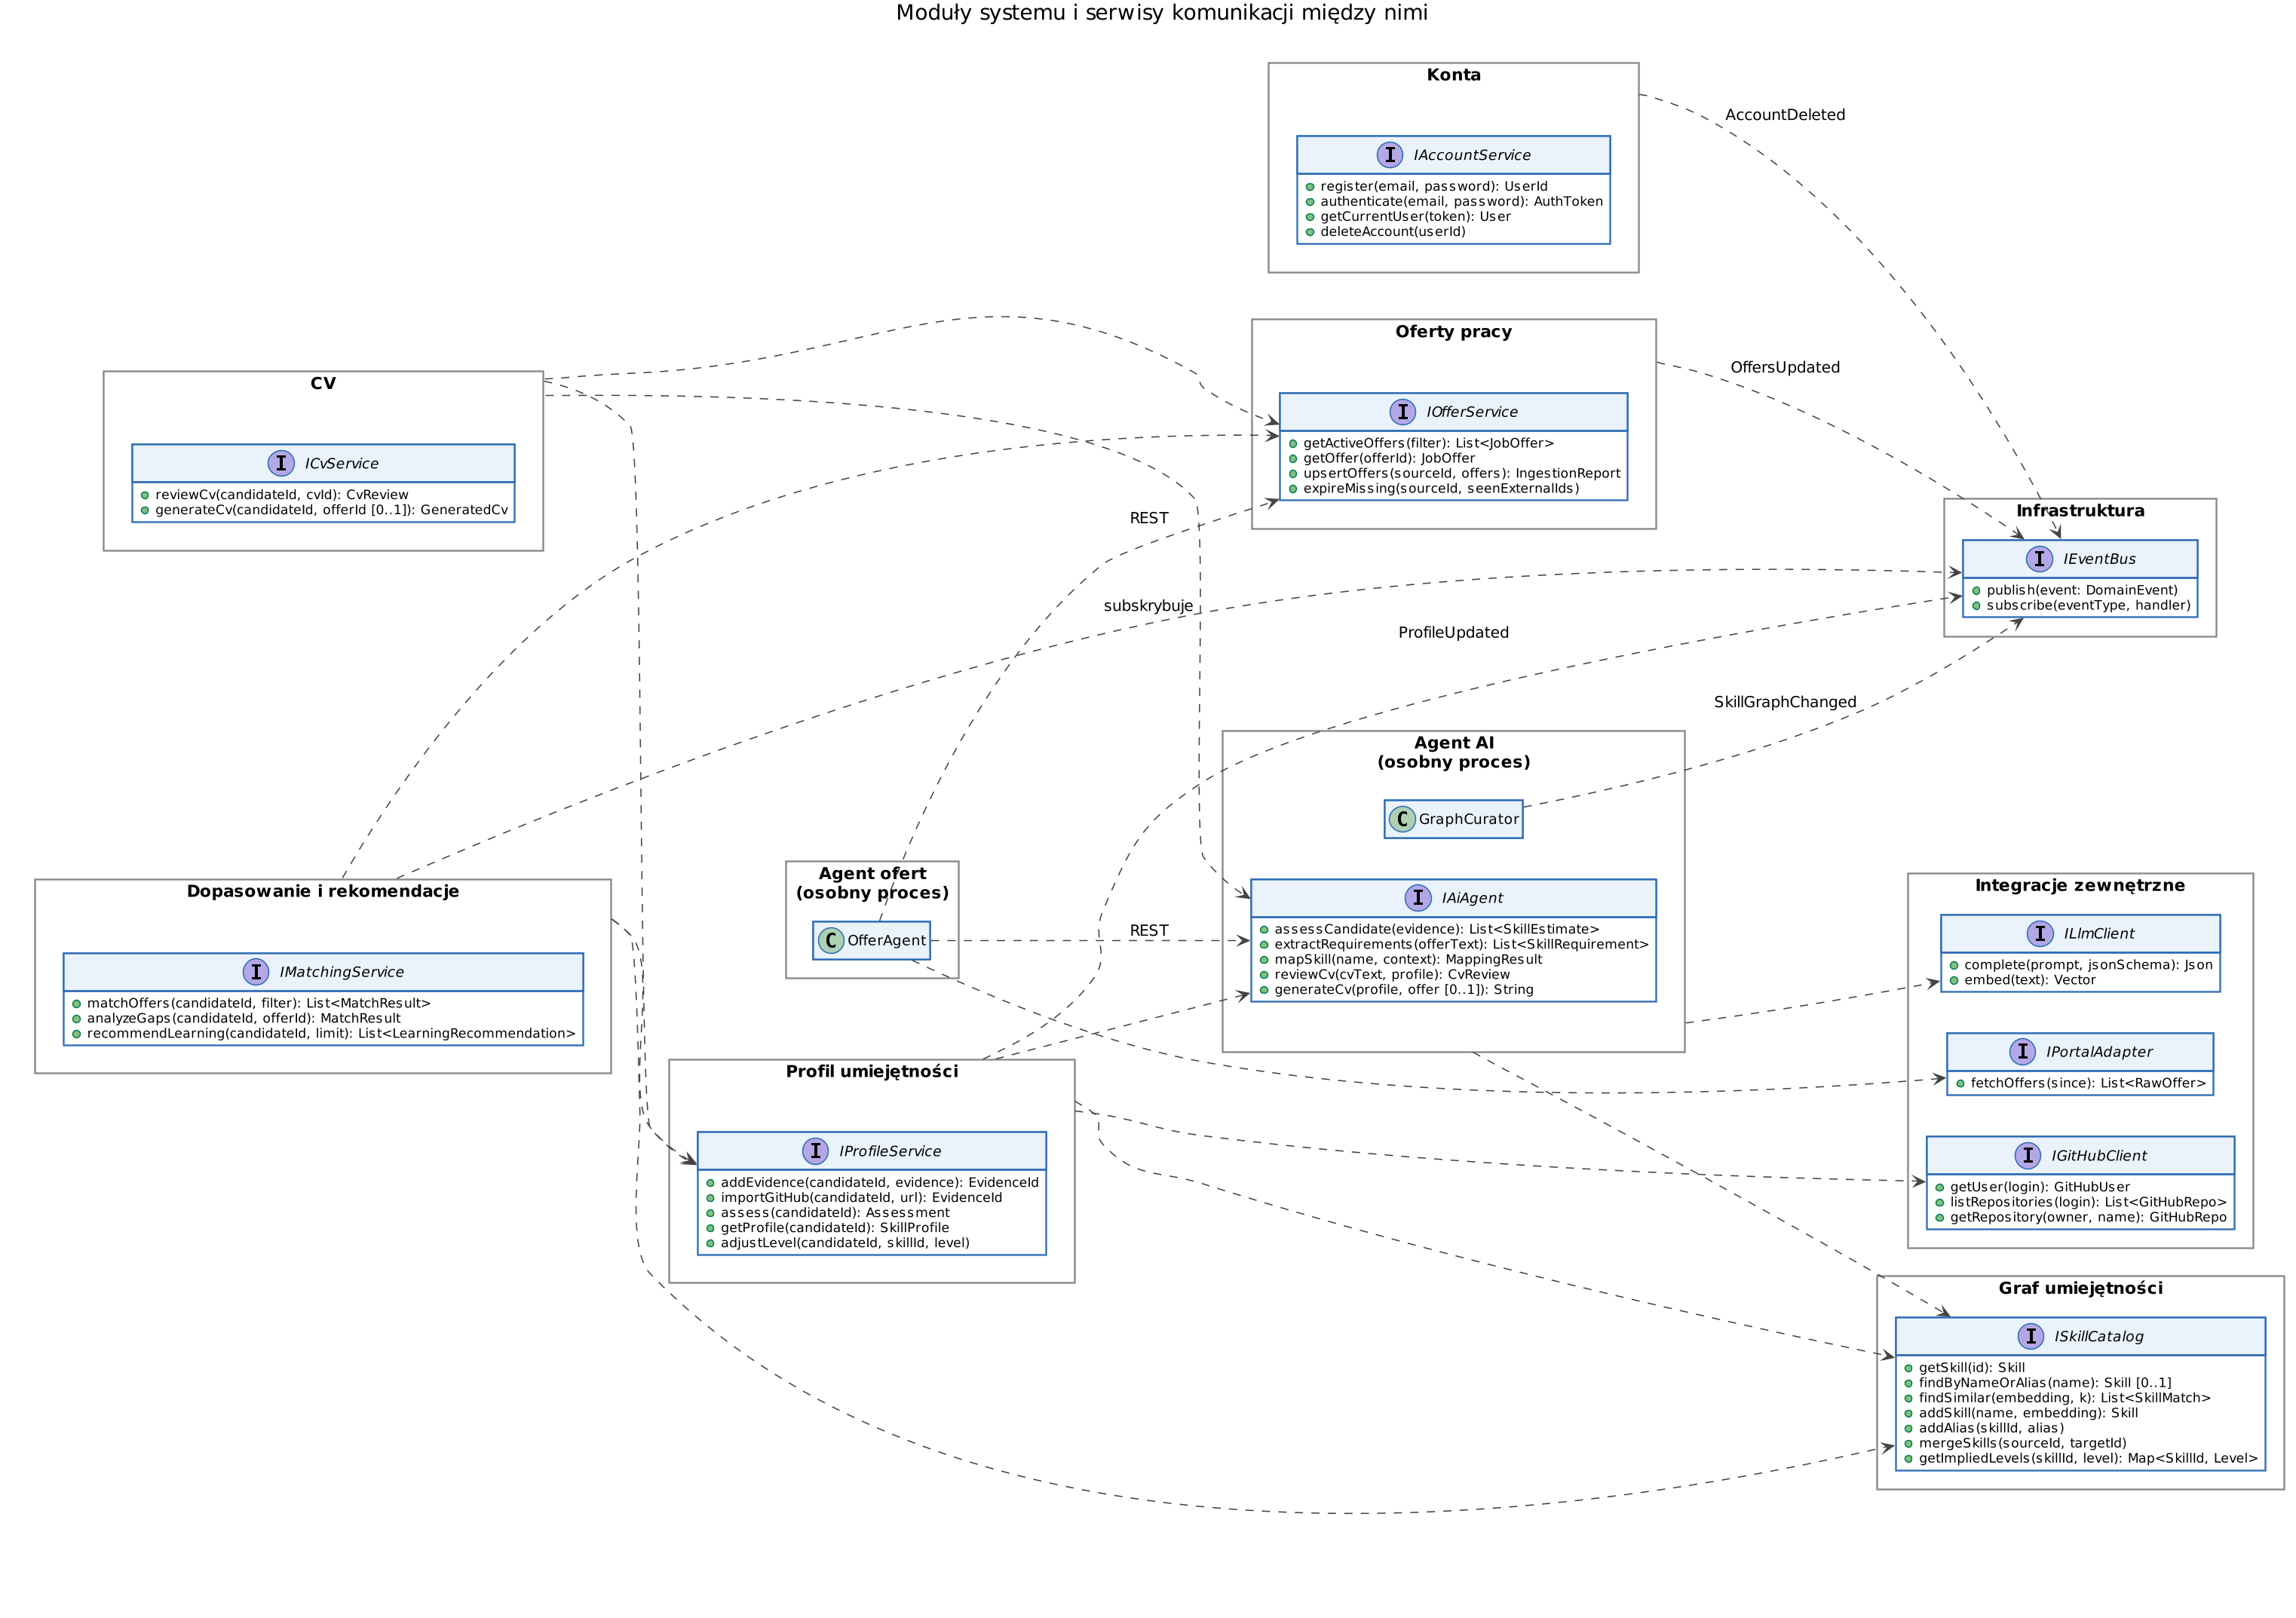
\includegraphics[width=\textwidth,height=0.86\textheight,keepaspectratio]{class-modules}
\end{frame}

\begin{frame}{Komunikacja między modułami}
  \small
  \begin{itemize}
    \item Moduły nie sięgają do cudzych danych --- tylko przez \alert{interfejsy serwisów}:
      \texttt{IProfileService}, \texttt{IOfferService}, \texttt{ISkillCatalog}, \texttt{IMatchingService}, \texttt{ICvService}, \texttt{IAiAgent}.
    \item Zmiany są ogłaszane \alert{zdarzeniami} na \texttt{IEventBus}:
      \texttt{ProfileUpdated}, \texttt{OffersUpdated}, \texttt{SkillGraphChanged}, \texttt{AccountDeleted}
      --- np. dopasowanie unieważnia wtedy swoją pamięć podręczną.
    \item \alert{Agent ofert} i \alert{Agent AI} to osobne procesy --- rozmawiają z serwerem przez REST.
    \item Tylko Agent AI rozmawia z modelem językowym (\texttt{ILlmClient}) --- zmiana dostawcy LLM nie dotyka reszty systemu.
    \item Każdy portal ma swój adapter (\texttt{IPortalAdapter}) --- dodanie portalu to nowa klasa.
    \item \alert{Graf umiejętności} jest wspólnym językiem: tymi samymi węzłami opisany jest profil i wymagania ofert.
  \end{itemize}
\end{frame}

\begin{frame}{Diagram klas --- graf i profil umiejętności}
  \centering
  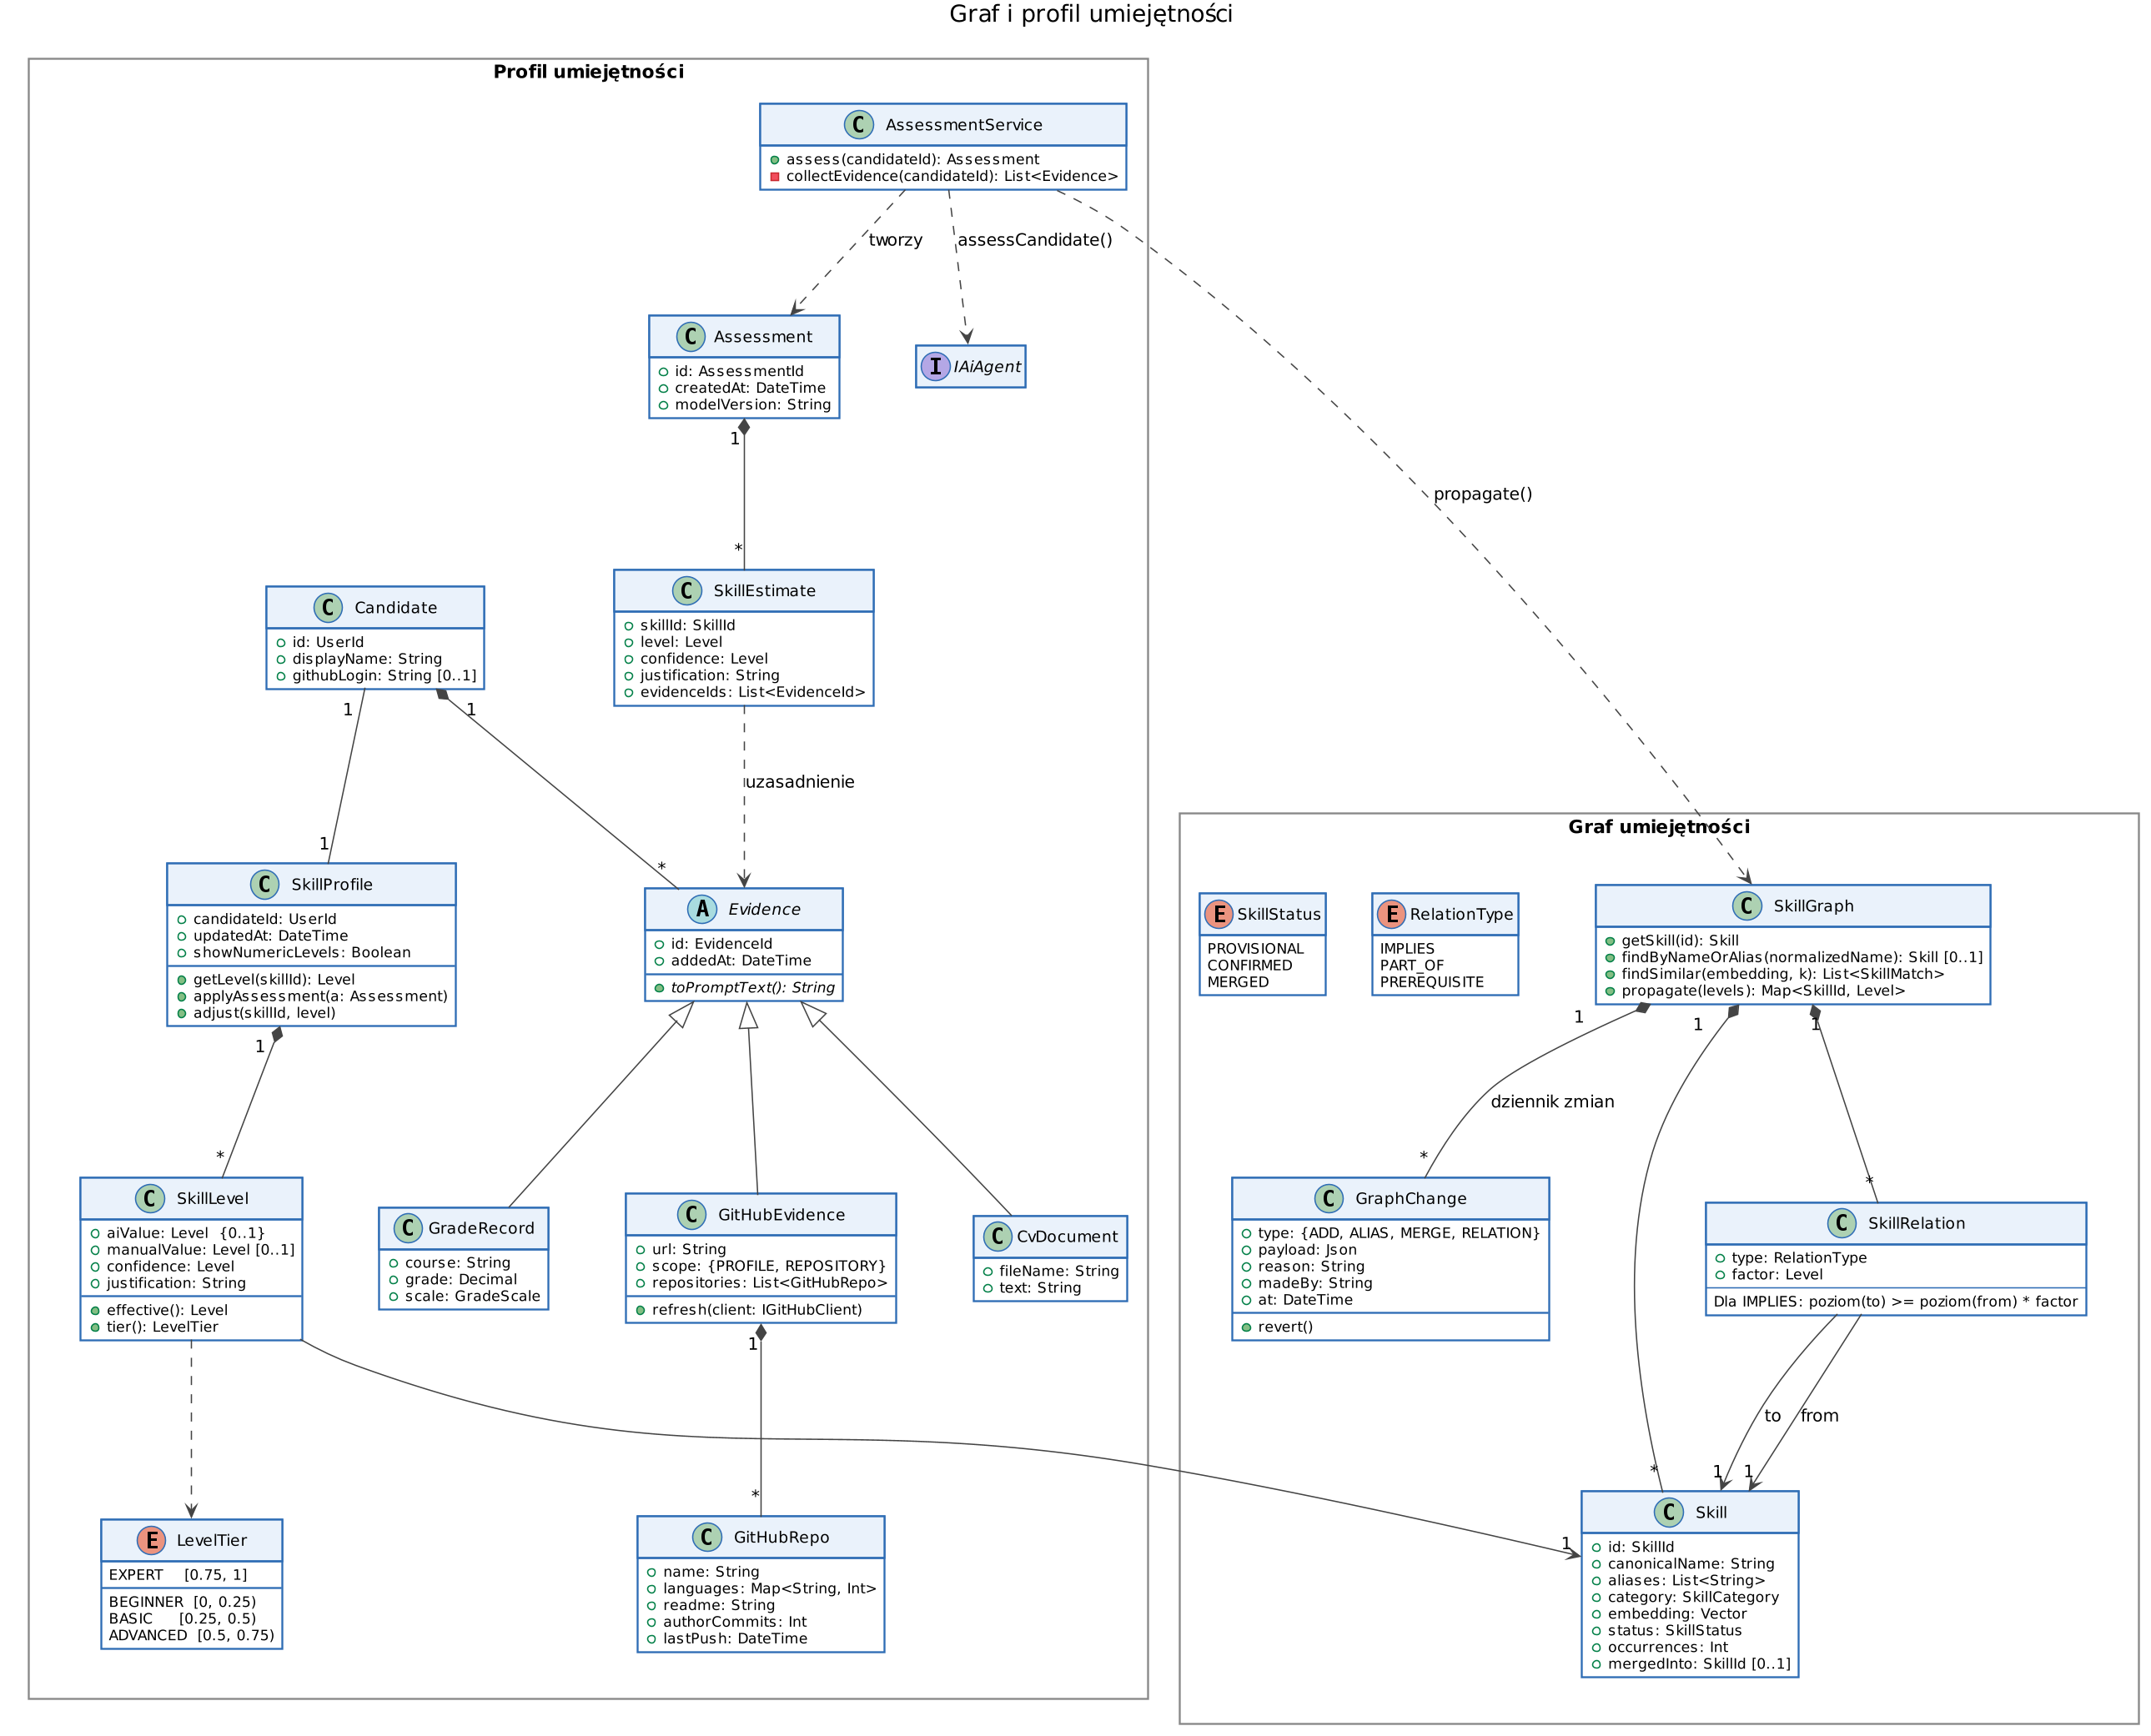
\includegraphics[width=\textwidth,height=0.86\textheight,keepaspectratio]{class-skills}
\end{frame}

\begin{frame}{Diagram klas --- Agent AI}
  \centering
  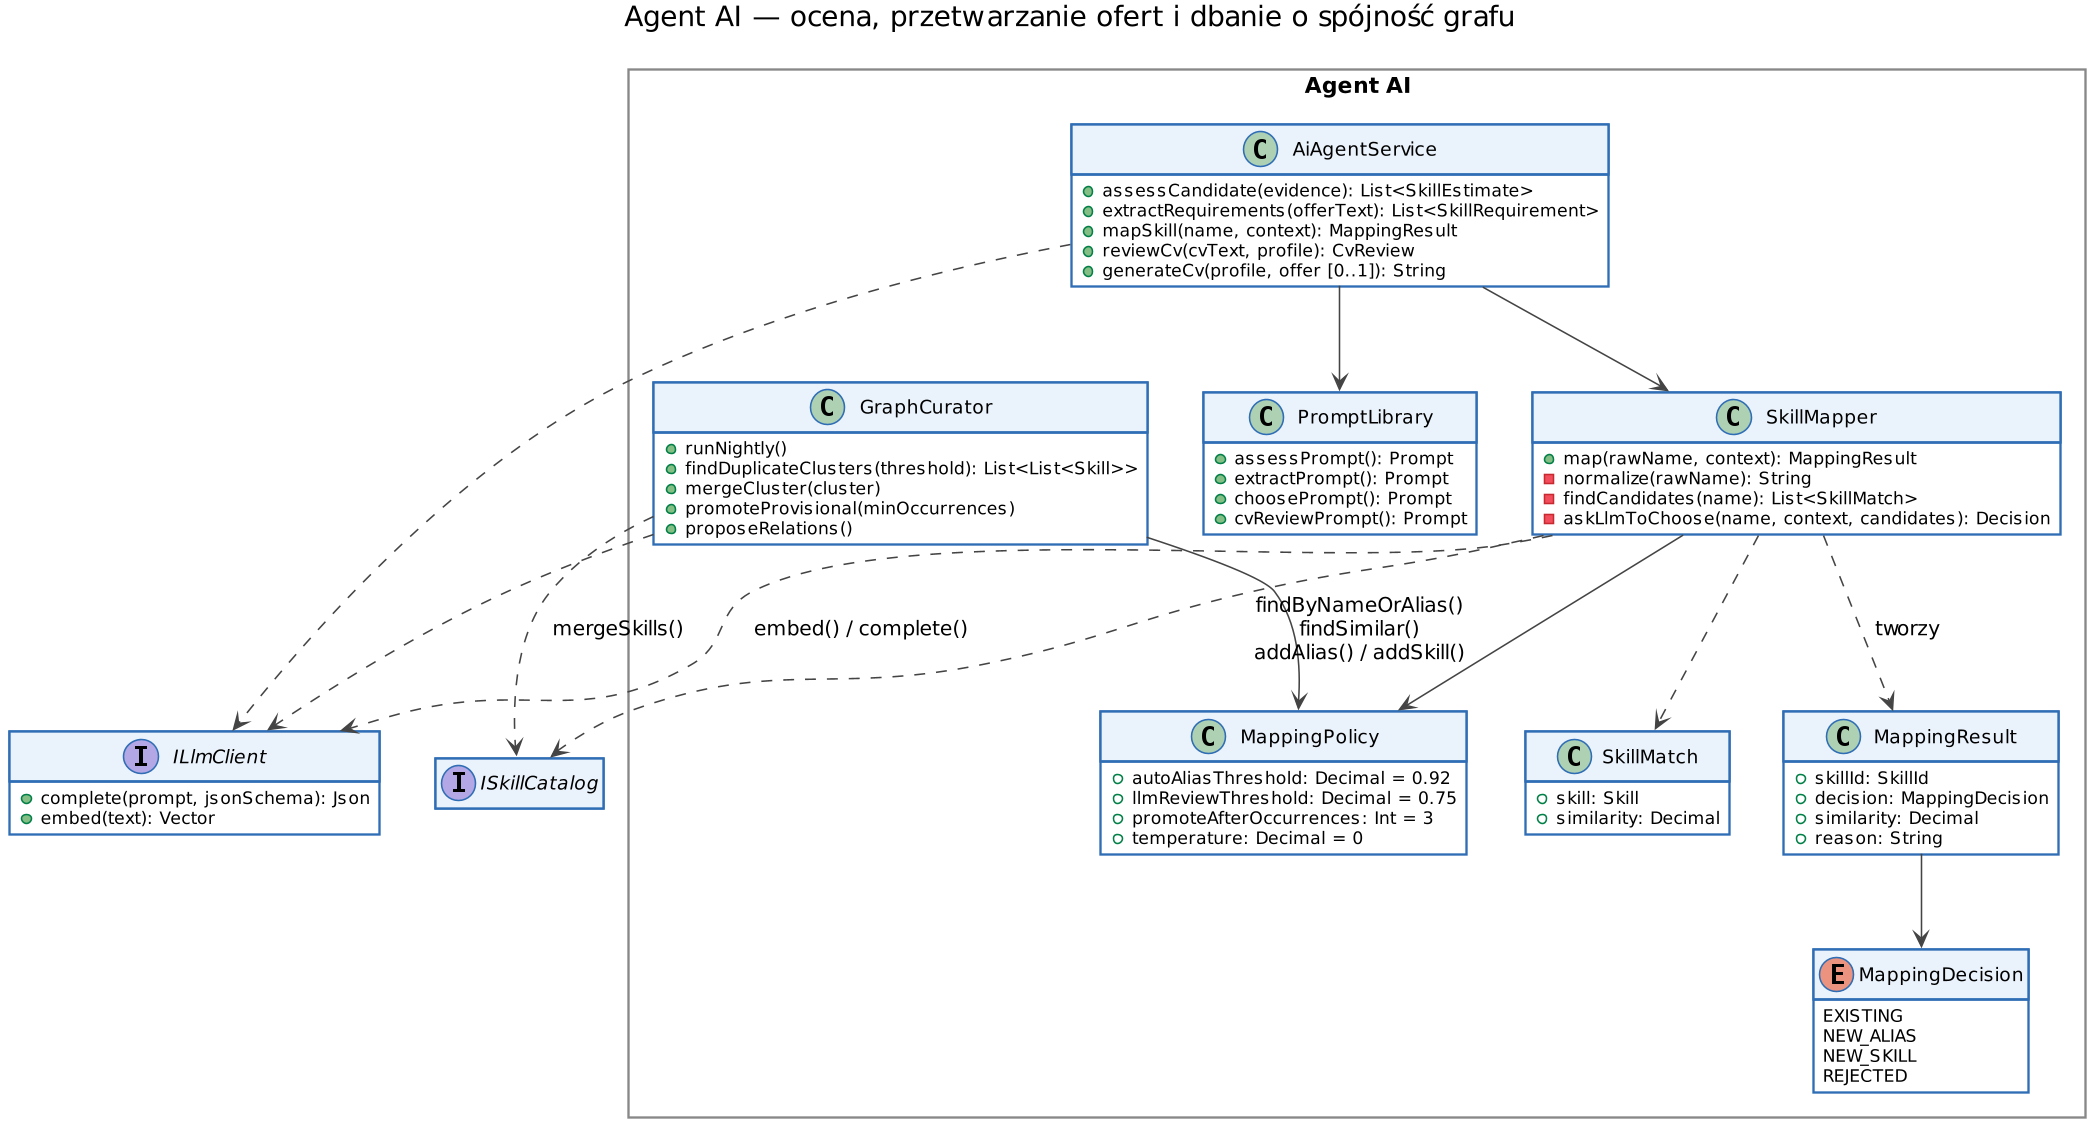
\includegraphics[width=\textwidth,height=0.86\textheight,keepaspectratio]{class-ai}
\end{frame}

\begin{frame}{Diagram klas --- oferty pracy i agent ofert}
  \centering
  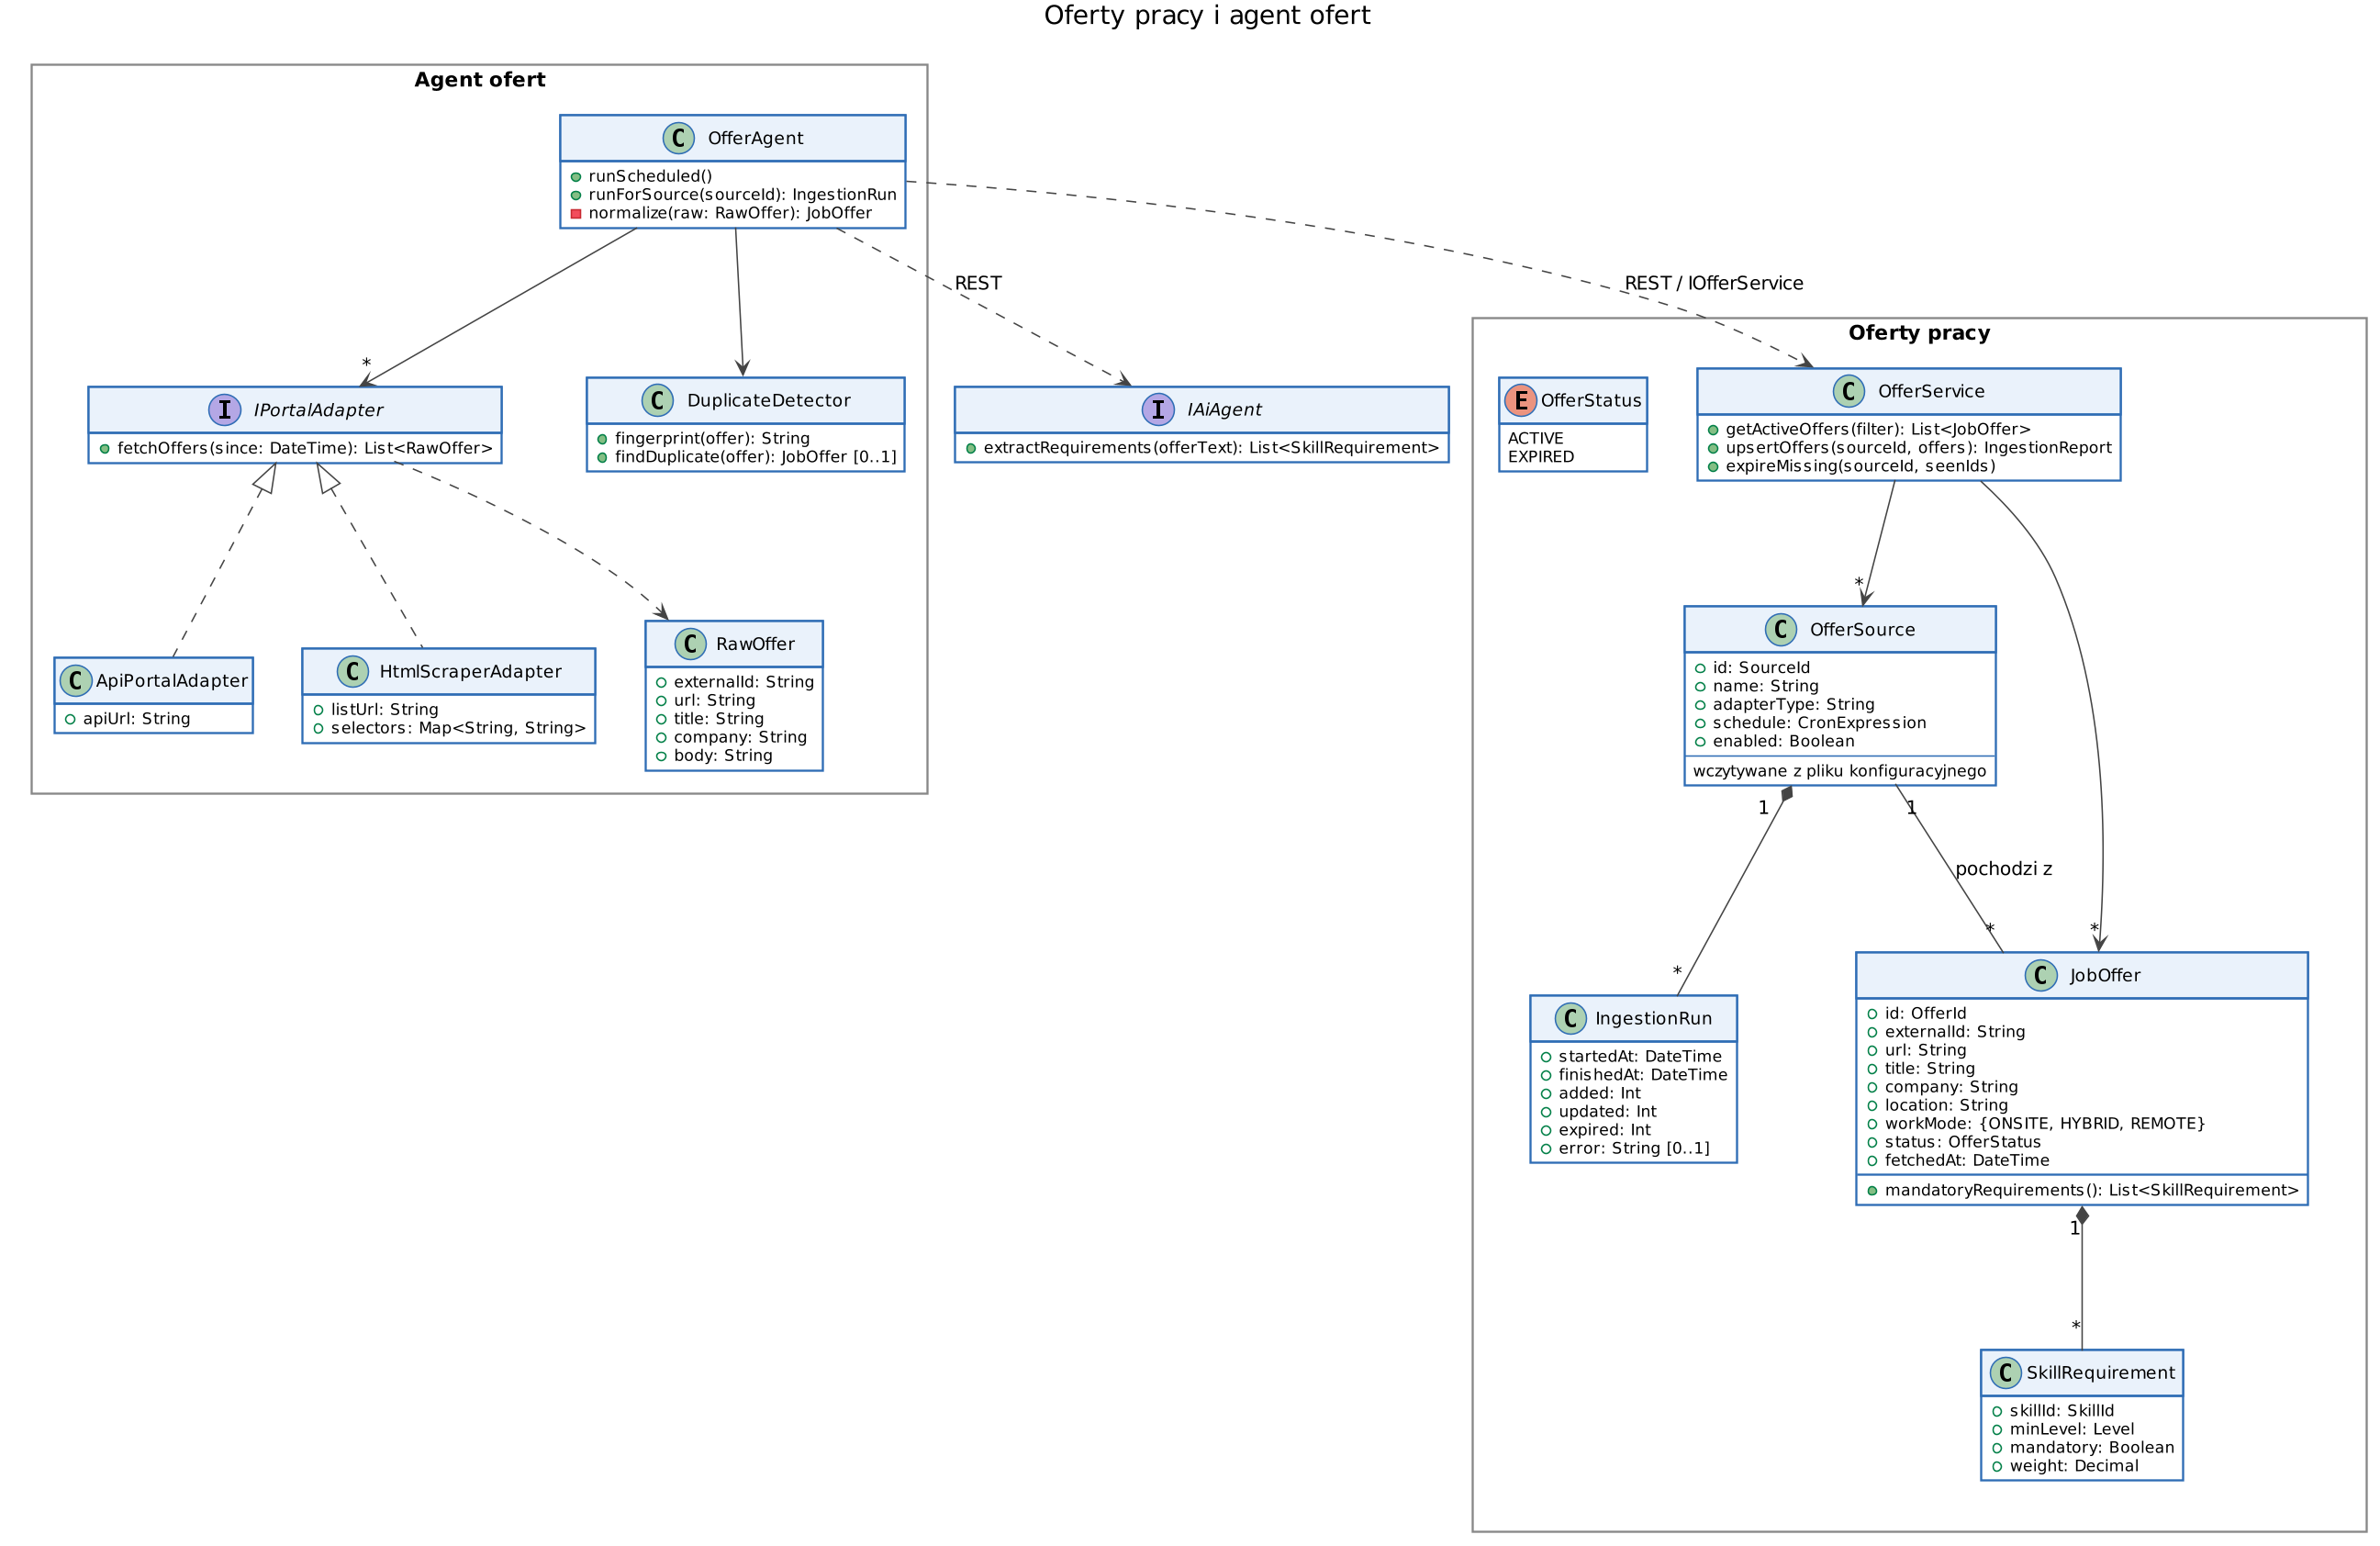
\includegraphics[width=\textwidth,height=0.86\textheight,keepaspectratio]{class-offers}
\end{frame}

\begin{frame}{Diagram klas --- dopasowanie, rekomendacje, CV}
  \centering
  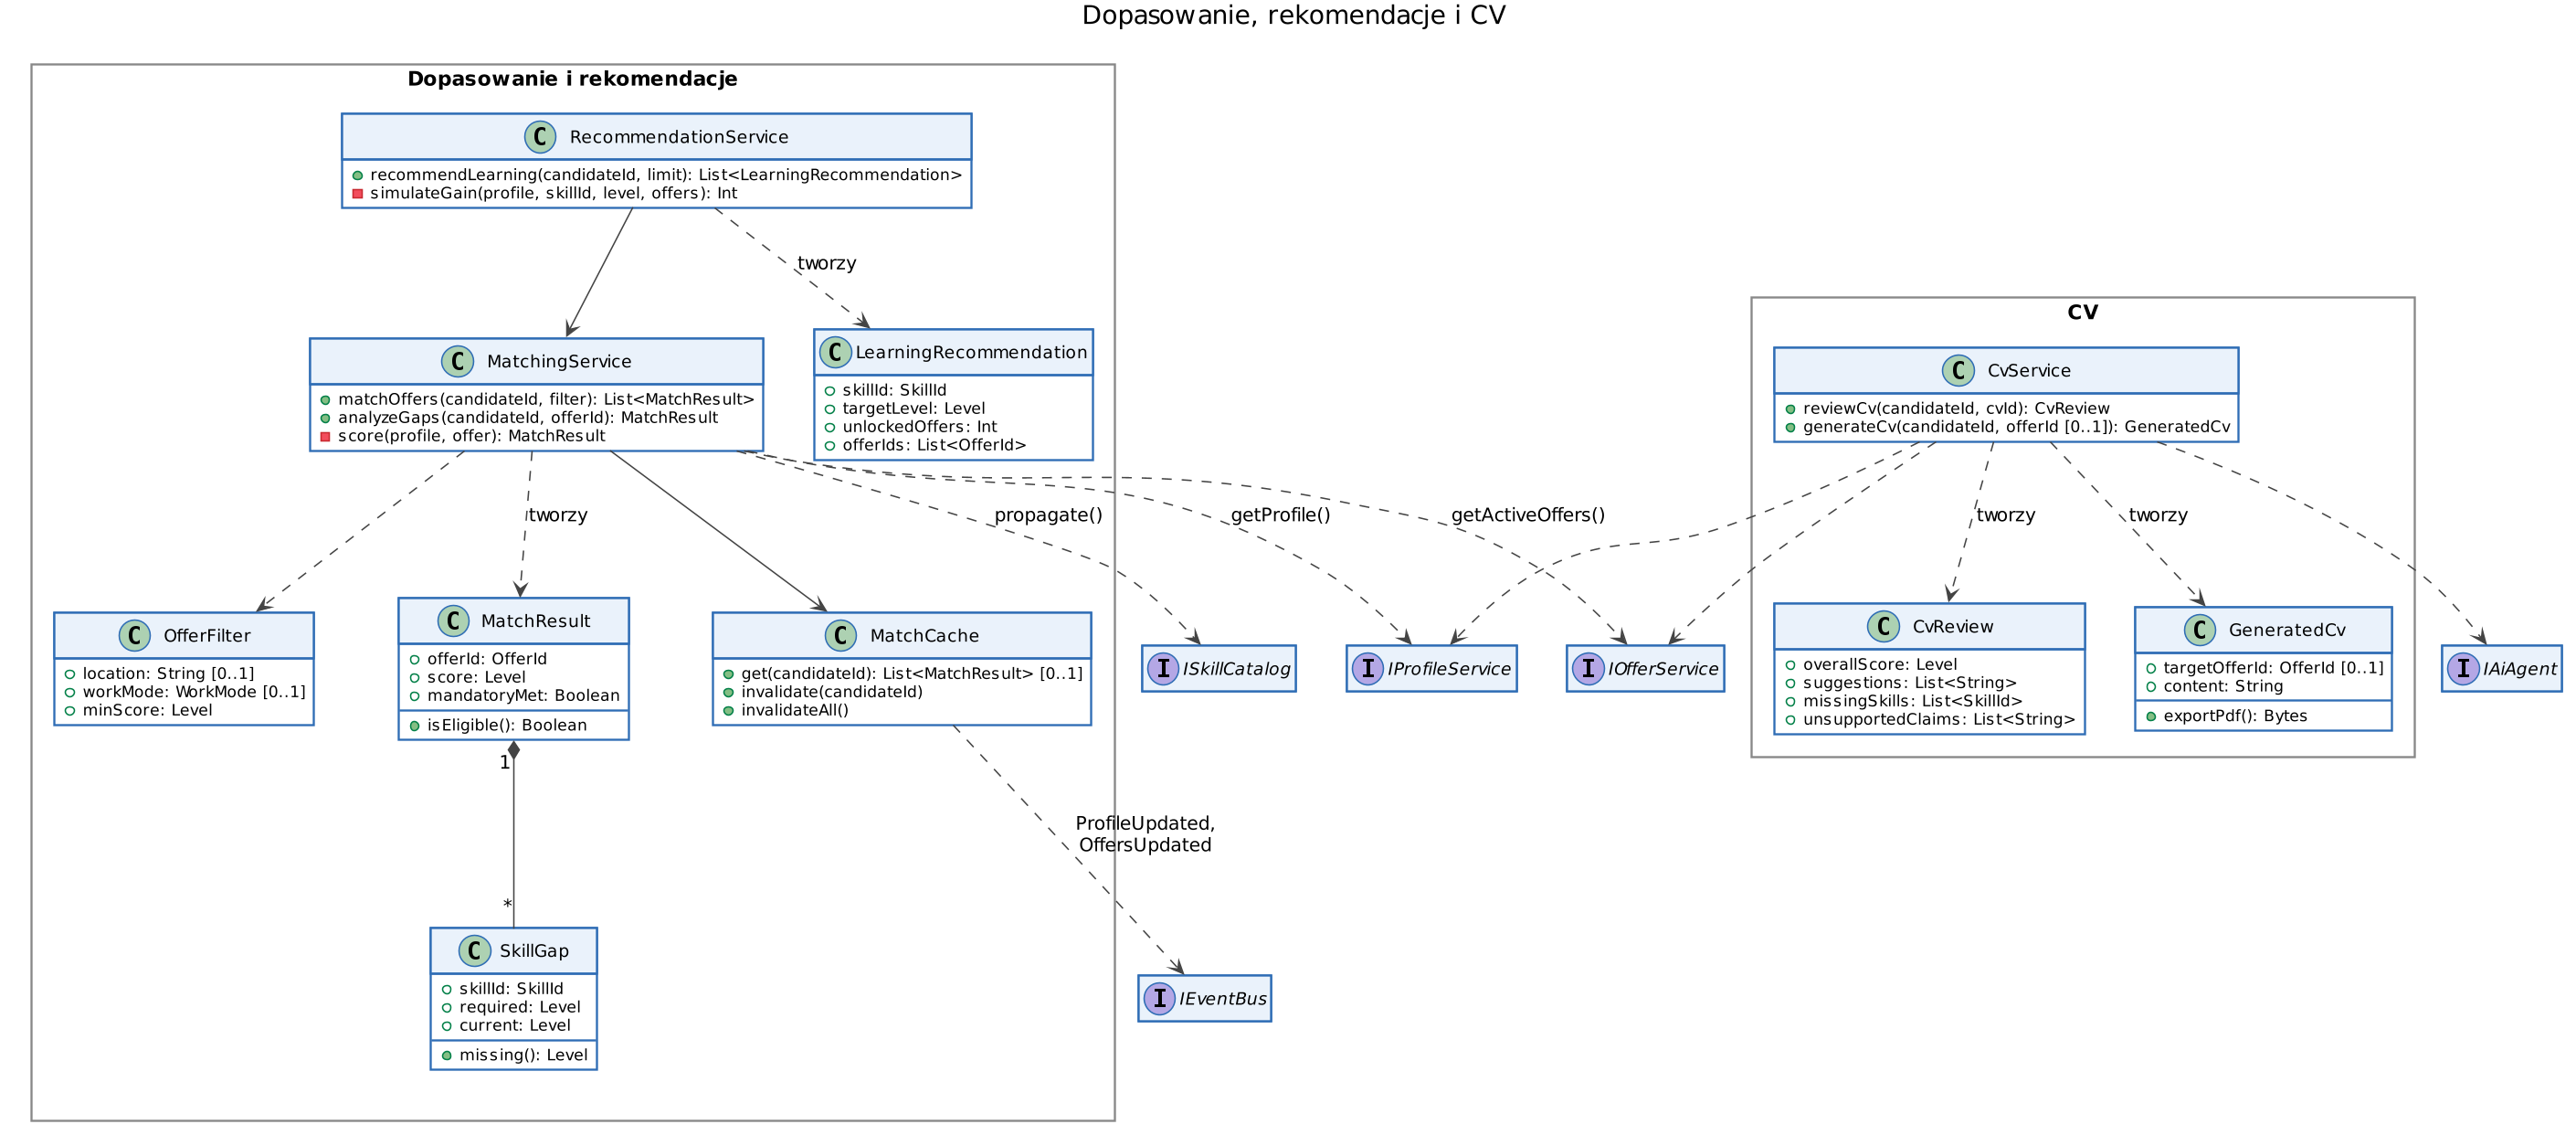
\includegraphics[width=\textwidth,height=0.86\textheight,keepaspectratio]{class-matching-cv}
\end{frame}

% ------------------------------------------------------------------
\begin{frame}{Otwarte pytania}
  \begin{itemize}
    \item Z których portali pobieramy oferty i czy ich regulamin na to pozwala (API vs scraping)?
    \item Jak sprawdzać jakość ocen AI --- ile ręcznych korekt to sygnał, że model się myli?
    \item Z jakiej klasyfikacji budujemy graf startowy (ESCO, tagi Stack Overflow, własna)?
    \item Jaki próg dopasowania uznajemy za „pasuje”?
  \end{itemize}
  \vfill
  \centering\Large Dziękujemy!
\end{frame}

\end{document}
